
\graphicspath{ {mainmatter/Kapur_2004/} }
\title*{2004: The Electronic Sitar Controller}
\titlerunning{Electronic Sitar Controller}


\author{Ajay Kapur, Ariel J. Lazier, Philip Davidson, R. Scott Wilson and Perry R. Cook}
\authorrunning{Kapur et al.}

%\institute{Ajay Kapur \at Department of Electrical and Computer Engineering, University of Victoria, Victoria, British Columbia, CANADA and Department of Computer Science, Princeton University, Princeton, New Jersey,  U.S.A., \email{ajay@ece.uvic.ca}
%\and Ariel  J. Lazier \at Department of Computer Science, Princeton University, Princeton, New Jersey,  U.S.A., \email{alazier@princeton.edu}
%\and Philip Davidson \at Department of Computer Science, Princeton University, Princeton, New Jersey,  U.S.A.
%\email{philipd@princeton.edu}
%\and R. Scott Wilson \at Center for Computer Research in Music and Acoustics, Stanford University, Stanford, California, U.S.A.
%, \email{rswilson@ccrma.stanford.edu}
%\and Perry R. Cook \at Department of Computer Science (also Music) Princeton University, Princeton, New Jersey,  U.S.A., \email{prc@cs.princeton.edu}}
%
%
\maketitle

\abstract*{This paper describes the design of an Electronic Sitar controller, a digitally
modified version of \textit{Saraswati's} (the Hindu Goddess of Music)
19-stringed, pumpkin shelled, traditional North Indian instrument. The
ESitar uses sensor technology to extract gestural information from a
performer, deducing music information such as pitch, pluck timing, thumb
pressure, and 3-axes of head tilt to trigger real-time sounds and graphics. It
allows for a variety of traditional sitar technique as well as new performance
methods. Graphical feedback allows for artistic display and pedagogical feedback.
The ESitar uses a programmable Atmel microprocessor which outputs
control messages via a standard MIDI jack.}

\section{Introduction}

The sitar is \textit{Saraswati's} (the Hindu Goddess of Music) 19-stringed,
pumpkin shelled, traditional North Indian instrument. Its bulbous gourd (shown in
Figure~\ref{Kapur:img-4}), cut flat on the top, is joined to a long necked hollowed concave stem
that stretches three feet long and three inches wide. The sitar contains seven
strings on the upper bridge, and twelve sympathetic stings below, all tuned by
tuning pegs. The upper strings include rhythm and drone strings, known as
\textit{chikari}. Melodies, which are primarily performed on the upper-most
string and occasionally the second string, induce sympathetic resonances in the
twelve strings below. The sitar can have up to 22 moveable frets, tuned to the
notes of a \textit{Raga} (the melodic mode, scale, order, and rules of a
particular piece of Indian classical music). The sitar is a very sophisticated
and subtle instrument, which can create vocal effects with incredible depths of
feeling, making it a challenging digital controller to create. \cite{Menon:1974,Vir:1998}


\begin{figure}[t]
\centering
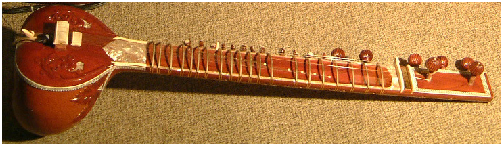
\includegraphics[width=\textwidth]{img-4-eps-converted-to-crop.pdf}      
\caption{A traditional Sitar.}
\label{Kapur:img-4}       % Give a unique label
\end{figure}

Our goal is to use sensor technology to extract musical information from a
performing sitar player, deducing gestural information such as pitch, thumb
pressure, and 3-axes of head tilt to trigger real-time sounds and graphics. In
this paper, we will present:

\begin{itemize}
	\item The evolution of the technology of the sitar from its origins until the present
day.
	\item The traditional playing style of the sitar, on which the controller is modeled.
	\item The creation of a real-time MIDI sitar
controller, using the Atmel microcontroller.
	\item The techniques used to map the signals captured from the sitar to sound{\large
.}
	\item The creation of a real-time graphical feedback system that reacts to the sitar
controller.
	\item The description of the sitar controller used in live performance.
\end{itemize}




\section{Evolution of the Sitar}

The precursor of the sitar is known as the \textit{vina}, of the lute family of instruments, which is referenced in Vedic writings as early as the first millennium B.C. Figure~\ref{Kapur:img-5} (a) shows an early version of the s\textit{tick zither vina,} from the 6$^{th}$ and 7$^{th}$ century A.D. From this picture it is evident that the \textit{stick zither }did not have frets, which ancient sculptures suggest evolved in the 10$^{th}$ and 11$^{th}$ Century A.D \cite{Bagchee:1998}. Figure~\ref{Kapur:img-5} (b) shows a primitive type of \textit{vina }instrument whose neck is made out of bamboo \cite{Sharma:1997}.


\begin{figure}[t]
\centering
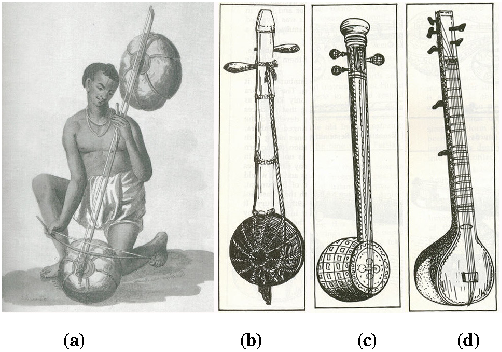
\includegraphics[width=\textwidth]{img-5-eps-converted-to-crop.pdf}      
\caption{(a) A \emph{stick zither vina} \cite{Bagchee:1998}, (b) A \emph{vina} made of
bamboo \cite{Sharma:1997}, (c) A \emph{sehtar} \cite{Sharma:1997}, (d) A 7-stringed sitar \cite{Sharma:1997}.}
\label{Kapur:img-5}       % Give a unique label
\end{figure}


There exist several differing historical accounts of the sitar's evolution. Some sources claim the instrument descended directly from the \textit{vina} as performers and builders made small modifications over time as technology and tools evolved. Others claim the similarity between the Middle-Eastern \textit{tambur} and the Persian s\textit{ehtar,} which traveled to India during the Muslim occupation of India in 11$^{th}$ century. The name seems to have derived from the Persian \textit{sehtar} (\textit{she}--three, \textit{tar}--strings) shown in Figure~\ref{Kapur:img-5} (c). In the 18$^{th}$ century, instrumentalist Amir Khusro is credited with adapting the name, as well as reversing the order of the strings, placing the main melody string to the far outside, thus making it easier for the performer to play with the instrument upright. \cite{Bagchee:1998} He also improved the sitar by making the frets movable (for fine tuning), by using string to tie the frets down. \cite{Sharma:1997}

In the 18$^{th}$ century, after the innovation of creating a wider bridge, four more strings were added to the sitar, giving a total of seven strings (as seen in Figure~\ref{Kapur:img-5} (d)). Other improvements include the introduction of metal frets and the \textit{mizrab}, the pyramid-shaped, wire plectrum. In the 19$^{th}$ century, the \textit{tarabdar} style of sitar emerged, which had 9 to 12 sympathetic strings (known as \textit{tarab)} positioned under the frets, as depicted in Figure~\ref{Kapur:img-4} \cite{Bagchee:1998}.


\begin{figure}[t]
\centering
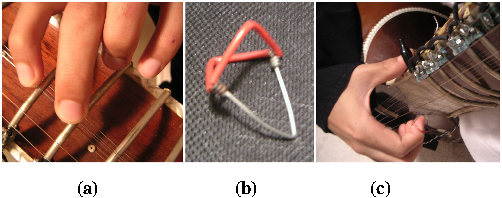
\includegraphics[width=\textwidth]{img-6-eps-converted-to-crop.pdf}      
\caption{Pictures showing sitar playing technique.}
\label{Kapur:img-6}       % Give a unique label
\end{figure}


In 2003, our team has brought the sitar
into the modern era of computers, adding resistors, capacitors, force sensing
resistors, microphones, and ethernet jacks, to enhance traditional technique with
the use of a laptop.

\section{Sitar Technique}

It is important to understand the traditional playing style of the sitar to comprehend how our controller captures its hand gestures. In this section, we will define the different parts of the sitar, briefly explain how North Indians annotate melodic notes, and describe the basic technique of sitar playing.

\subsection{Construction of a Sitar}

The gourd section of the sitar is known as the \textit{tumba} and plays the role of a resonating chamber. The flat piece of wood which lays on the front side of the \textit{tumba} is known as the \textit{tabli. }The long column which extends from the \textit{tumba} is known as the \textit{dand }(similar to the neck of a guitar)\textit{, }and is made out of the same material as the \textit{tabli}. This part of the instrument acts as a column resonator. Sometimes, a second \textit{tumba} is put at the \textit{dand} to increase resonance.

The seven main upper strings run along the \textit{dand}, above moveable, curved metal frets, over a bridge (\textit{jawari)} made of ivory or deer horn and tie together at the \textit{langot }at the very bottom of the sitar. The sympathetic strings, or \textit{tarab} strings, run below the frets and have their own separate bridge \textit{(ara)}, but still tie together at the \textit{langot.} All strings are made of steel, except for the second upper string (right next to the main melody string), which is made of copper.

\subsection{Hindustani Note Annotation}

There are seven main notes (\textit{swara)} in Hindustani music: \textit{Shadja}
(\textit{Sa}), \textit{Rishab} (\textit{Re}), \textit{Gandhar} (\textit{Ga}),
\textit{Madhyam} (\textit{Ma}), \textit{Pancham} (\textit{Pa}), \textit{Dhaivat}
(\textit{Dha}), and \textit{Nishad} (\textit{Ni}). These seven notes correspond
directly with the western \textit{Do}, \textit{Re}, \textit{Mi}, \textit{Fa},
\textit{So}, \textit{La}, \textit{Ti}, and represent the seven notes in a major
scale. Octaves are indicated with a mark as follows: \textit{Sa$_{o}$} (lower
octave), \textit{Sa} (middle octave), \textit{Sa$^{o}$} (upper octave).
\textit{Re}, \textit{Ga}, \textit{Dha}, and \textit{Ni}, have notes which are
half step below, known as \textit{komal}, and are represented as follows:
\textit{\underline{Re}}, \textit{\underline{Ga}}, \textit{\underline{Dha}},
\textit{\underline{Ni}}. The note in between Ma and Pa, (known as a tri-tone in 
Western music) is known as \textit{tivra} \textit{Ma}. There are more notes in
between these twelve basic notes, known as \textit{shruti,} which translate to
microtones. These notes are traversed when transitioning from one main note to
another. There is no agreed-upon method of transcribing \textit{shruti}, and
proper technique can only be learned in a traditional \textit{guru} (master) to
\textit{shishak}  (student) tutoring. \cite{Bagchee:1998,Sharma:1997,Vir:1998}

\subsection{Sitar Playing Technique}

It should be noted that there are two main styles of sitar technique: Ustad
Vilayat Khan's system and Pandit Ravi Shankar's system. The main differences
between the styles are that Ustad Vilayat Khan performs melodies on the higher
octaves, eliminating the lowest string from the instrument, whereas Pandit Ravi
Shankar's style has more range, and consequently melodies are performed in the
lower octaves \cite{Bagchee:1998}. The ESitar is modeled based on the Vilayat Khan
system.

A performer generally sits on the floor, in a cross-legged fashion. Melodies are
performed primarily on the outer main string, and occasionally on the copper
string. The sitar player uses his left index finger and middle finger, as shown
in Figure~\ref{Kapur:img-6}(a), to press the string to the fret for the desired \textit{swara.}
In general, a pair of frets are spaced a half-step apart, with the exception of a
few that are spaced by a whole step (typically around \textit{Sa }and
\textit{Pa}).\textit{ }The frets are elliptically curved so the string can be
pulled downward, to bend to a higher note. This is how a performer incorporates
the use of \textit{shruti }(microtones).

On the right index finger, a sitar player wears a ring like plectrum, known as a
\textit{mizrab, }shown in Figure~\ref{Kapur:img-6}(b)\textit{. }The right hand thumb, remains
securely on the edge of the \textit{dand} as shown on Figure~\ref{Kapur:img-6}(c), as the entire
right hand gets pulled up and down over the main seven strings, letting the
\textit{mizrab }strum the desired melody. An upward stroke is known as
\textit{Dha }and a downward stroke is known as \textit{Ra. } \cite{Bagchee:1998,Vir:1998}

\section{The  MIDI  sitar controller.}

With the goal of capturing a wide variety of gestural input data, the
ESitar controller combines several different families of sensing
technology and signal processing methods.  These are broken down into the
microcontroller platform, in Section 4.1 and the individual gestures and their
corresponding sensors and algorithms in Section 4.2.

\subsection{The Atmel microcontroller.}

The core of the ESitar's sensing and communication systems is an Atmel
AVR ATMega16 microcontroller. The microcontroller is exploited primarily for its
several parallel on-board analog to digital converters \cite{Wilson:2003}.  As the various
sensor inputs are digitized by the microcontroller we do some pre-processing of
the resulting signals to clean them up and/or classify them before forwarding
them on to the host computer via MIDI.


\begin{figure}[t]
\centering
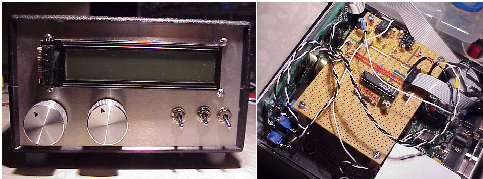
\includegraphics[width=\textwidth]{img-7-eps-converted-to-crop.pdf}      
\caption{The controller box.}
\label{Kapur:img-7}       % Give a unique label
\end{figure}


The Atmel is encased in a controller box as seen in Figure~\ref{Kapur:img-7}, with a number
switches, shaft encoders, and potentiometers used to trigger events, toggle
between modes, and fine tune settings. The box also has an LCD to display
controller data and settings to the performer, enabling him/her to be completely
detached from the laptops running sound and graphic simulations. The sitar and
headset are each connected to the main control box using Ethernet type patch
cables. These cables provide a clean and robust interconnection over which the
analog sensor signals are sent to the control hardware.

\subsection{Gesture Capturing}

The specific gestures our system captures data from are the depressed fret
number, pluck time, thumb pressure, and 3 axes of the performer's head tilt.

\subsubsection{Monophonic pitch detection.}

The currently played fret is deduced using an exponentially distributed set of
resistors which form a network interconnecting in series each of the frets on the
ESitar (pictured in Figure~\ref{Kapur:img-11}).  When the fingers of the left hand
depress the string to touch a fret (as shown in Figure~\ref{Kapur:img-6}(a)), current flows
through the string and the segment of the resistor network between the bottom and
the played fret. The voltage drop across the in-circuit segment of the resistor
network is digitized by the microcontroller. Using a lookup table it maps that
value to a corresponding fret number and sends it out as a MIDI message.


\begin{figure}[t]
\centering
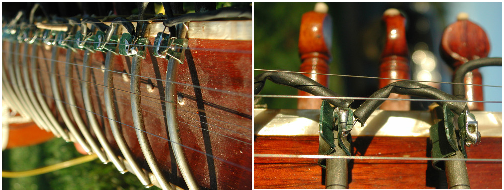
\includegraphics[width=\textwidth]{img-11-eps-converted-to-crop.pdf}      
\caption{Network of resistors on the frets of the ESitar.}
\label{Kapur:img-11}       % Give a unique label
\end{figure}

\begin{figure}[t]
\centering
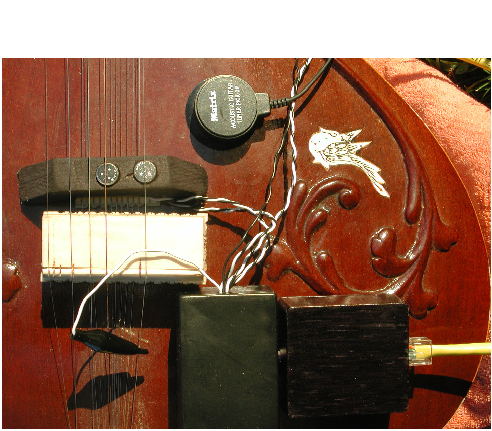
\includegraphics[width=78mm]{img-1-eps-converted-to-crop.pdf}      
\caption{Gesture capturing sensors at base of the ESitar.}
\label{Kapur:img-1}       % Give a unique label
\end{figure}


As mentioned above, the performer may
pull the string downward, bending a pitch to a higher note (for example play a
\textit{Pa }from the \textit{Ga} fret). To capture this additional information
that is independent of the played fret, we fitted the instrument with a piezo
pick-up to be fed into a pitch detector.  We chose to implement the pitch
detector as a Pure Data \cite{Puckette:1996a} external object using an auto-correlation
based method \cite{Zolzer:2002}.  The pitch detection is bounded below by the pitch of the currently played fret and allows a range of eight semi-tones above.

\subsubsection{Mizrab Pluck Time}

Pluck time is derived using two condenser microphones placed on a third bridge
above the \textit{ara }(shown in Figure~\ref{Kapur:img-1}). The microphones are located directly
under the main melody string and the copper string. The signals from the
microphones are passed through an analog envelope detector to extract the pluck
time. We also use these microphones to determine on which string the melody is
being played. If the melody is being played on the copper\textit{ }string (which
is very rare), we can safely assume that the main melody string is not being
played. The microcontroller sends a MIDI message when a pluck occurs, embedding
the information for the string that was plucked.

\begin{figure}[t]
\centering
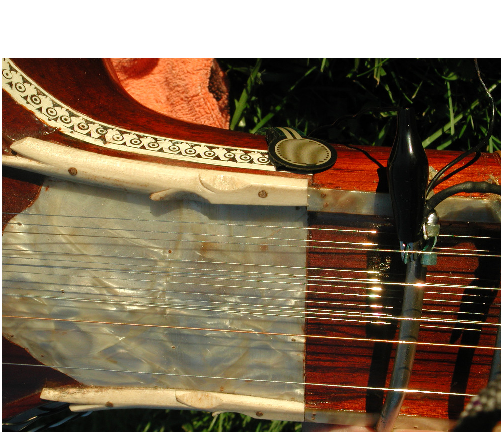
\includegraphics[width=78mm]{img-2-eps-converted-to-crop.pdf}      
\caption{FSR sensor used to measure thumb pressure.}
\label{Kapur:img-2}       % Give a unique label
\end{figure}


\subsubsection{Mizrab Pluck Direction}

We are able to deduce the direction of a \textit{mizrab} stroke using a force
sensing resistor (FSR), which is placed directly under the right hand thumb, as
shown in Figure~\ref{Kapur:img-2}. As mentioned before, the thumb never moves from this position
while playing. However, the applied force varies based on \textit{mizrab} stroke
direction. A \textit{Dha }stroke (upward stroke) produces more pressure on the
thumb than a \textit{Ra} stroke (downward stroke). We send a continuous stream of
data from the FSR via MIDI, because this data is rhythmically in time and can be
used compositionally for more then just deducing pluck direction.


\begin{figure}[t]
\centering
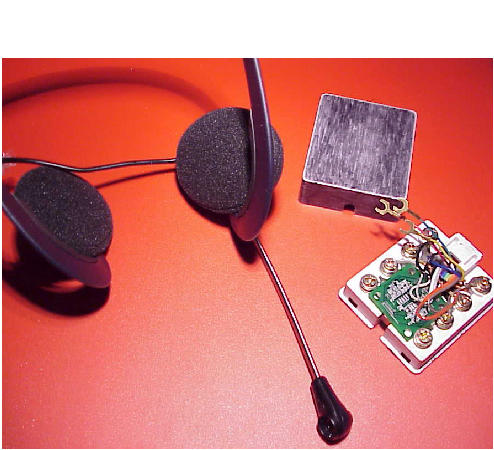
\includegraphics[width=78mm]{img-3-eps-converted-to-crop.pdf}      
\caption{Headset with accelerometer chip.}
\label{Kapur:img-3}       % Give a unique label
\end{figure}


\subsubsection{3-Axes Head Tilt}

An accelerometer is attached to a headset (as shown in Figure~\ref{Kapur:img-3})  in order to
obtain 3-axes of head tilt information. We see the head as an easy way to control
and trigger different events in the performance \cite{Merrill:2003}. We send continuous head data
out via MIDI messages. The headset would be a useful addition to almost any
controller as a replacement for foot pedals, buttons, or knobs. It is
particularly useful in this system as a sitar player's hands are always busy, and
cannot use his/her feet due to the seated posture.

\section{Mapping Signals to Sound}

Once we have control information describing pitch, pluck time, pluck
direction/power, and head tilt, we must decide how to use this information to
create sound.

\subsection{Requirements}

The ESitar produces the natural sound of the instrument as well as
control information. Thus, we must take care that the sounds we produce
complement the acoustic sound of a classical sitar. This task is possible because
of the detailed information available about what is being played. There are two
classes of electronic sounds we can produce. The first consists of sounds that
function as an extension of an acoustic sitar. One means of extending the sound
of the sitar is to simply process the signal coming through a pickup with
standard effects such as delay and reverb. This is trivial because there is no
need for the detailed information regarding the musician's interaction with their
instrument to apply these effects. With very accurate information to describe the
actions of the sitar player it is possible to create effects that reach beyond
basic processing of the acoustic sitar sound. When attempting to extend the sound
of the sitar, we must take care that the mapping of control information to sound
is done in such a way that the performer can control both the acoustic sound and
synthesized sound simultaneously. Such mappings can be considered a coupling of
the gestures used to create the acoustic and electronic sounds. Recent research
has shown that such mappings have the potential to be more expressive and
powerful than one to one mappings between control information and synthesis
parameters \cite{Hunt:2002}. The second class of electronic sounds we can produce consists of
sounds that function as counterpoint to the sound of the sitar. This class of
sounds focuses more on the analysis of control information and the creation of a
computerized accompaniment or response, rather than mapping control parameters
directly to sound. To interact with such a system, the performer does not try to
trigger control information, but instead varies their interaction with the
acoustical instrument to implicitly direct the computer-generated sounds.  For
example, with the detailed information available, it is possible to generate
tabla beats that correctly complement and react to the acoustic sound of the
sitar.

\subsection{Pure Data Patches}

All of the signals generated by the ESitar are sent into a computer and
captured by Miller Puckette's Pure Data program \cite{Puckette:1996a}. This information
could be used in many other ways, but we chose to use \textit{pd} because of the
ease of capturing and manipulating the control information within the \textit{pd}
environment. Below, we describe a number of different Pure Datapatches
written to demonstrate how such control information can be used.

\subsubsection{Slide Sitar}

The slide sitar patch was modeled after the sound of a slide guitar. It is a
simple module that consists of a bank of oscillating comb filters. The filters
have a resonance that is determined by the frequency indicated by the fret
information. The control information is used to change the resonance of the
filters. We also use thumb pressure to control the amplitude of the resonance
oscillation. Here we interpret thumb pressure as a measure of intensity of the
performance. The intensity of each pluck can be heard through the amplitude of
the filters' oscillations. This is a very simple use of the control information,
but such an effect could not be obtained without the detailed information
provided by the ESitar.

\subsubsection{Sympathetic pitch}

The sympathetic pitch patch plays rolls of a sampled sitar sound at the pitch
indicated by the fret. In this case we mapped thumb pressure to the volume of the
roll and head tilt to length of the notes and speed of the roll. Because the
sounds produced do not directly correspond to the acoustic sound, this is more of
a complementary patch. This is apparent when the performer increases the pressure
on the thumb FSR on a beat where the strings are not strummed. In these instances
the roll becomes more prominent and can function as a rhythmic replacement for
the sitar when the acoustic sound is not heard.

\subsubsection{Ring Modulation and Delay}


\begin{figure}[t]
\centering
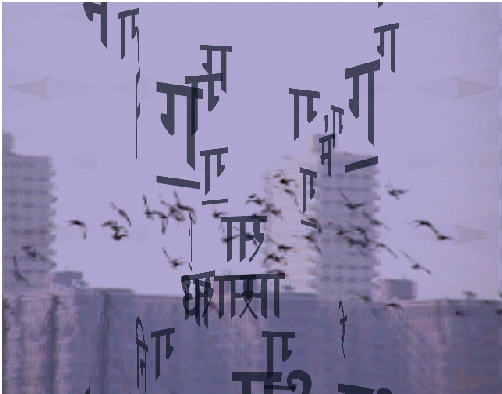
\includegraphics[width=78mm]{img-8-eps-converted-to-crop.pdf}      
\caption{A roll of \textit{swara} rendered over video stream.}
\label{Kapur:img-8}       % Give a unique label
\end{figure}



This patch also takes into account the
fret information, setting the frequency of the modulation to the pitch indicated
by the frets. This patch produces a distorted sound that would not be possible to
create without the accurate pitch information provided by the controller. We also
set up a delay system controlled by the head and the thumb. The system allows the
musician to capture parts of the output of the ring synthesis module into a loop
for later playback and combination with other loops. The head tilt controls which
loops are played or filled with new sound, while the thumb controls if or how
much sound should be played or stored into the loop buffers.

\subsubsection{Analysis/Re-Synthesis}


\begin{figure}[t]
\centering
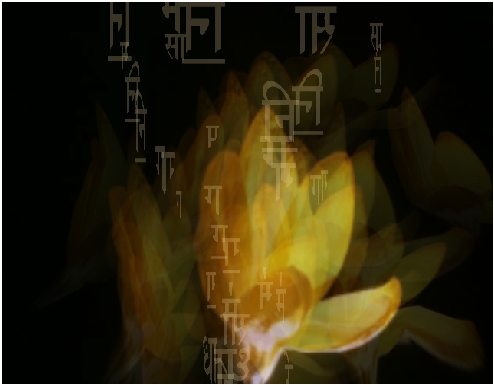
\includegraphics[width=78mm]{img-9-eps-converted-to-crop.pdf}      
\caption{Animation scrubbing from thumb pressure.}
\label{Kapur:img-9}       % Give a unique label
\end{figure}


Our last example is a simple
analysis/re-synthesis patch. We use fret information and pitch information to
identify which partials are generated by the struck note. Simply taking the
strongest partials would not lead to the same results because of the sympathetic
strings that are constantly resonating. Once the strongest partials are chosen,
sine waves with very short envelopes are synthesized which together form a
disjointed representation of the acoustic sitar sound. The volume of the
re-synthesis is scaled to the sound of the acoustic sitar and then controlled by
head tilt. We warp the volume distribution of the detected partials using thumb
pressure. When greater thumb pressure is applied, the lower partials are given
more weight and are more easily discernable.

\subsubsection{Drone}

We also added the capability to control the sound of a drone using head tilt.
The drone is created using a bank of fm synthesizers. Each of the synths are
tuned to \textit{Sa} or \textit{Pa}, each with a different set of harmonics. They
are also specialized so that head tilt controls the relative loudness of each of
the synths. This gives the performer the ability to control which synths are most
prominent.

\section{Graphic Feedback}

We rendered the visuals for the ESitar performance using
\textit{veldt} \cite{Kapur:2003}, as our visual design environment, and we chose to model our
visualization on the traditional form of melodic notation for sitar. As the
player performs, we read the incoming note/velocity pairs from the Atmel chip to
render a stream of \textit{swara}, which are arranged in a helix as if they are
printed on spinning drum of paper (shown in Figure~\ref{Kapur:img-8}).  We use a discrete rhythm
detection algorithm \cite{Dixon:2000} over a recent history of notes played to estimate a rough
beat-per-minute value, which modulates the speed at which the drum rotates so
that one measure is displayed per rotation of the drum.  Notes played with
greater intensity are rendered in a larger, bolder style, emphasizing them within
the overall display. Rhythmic patterns are reflected visually as symmetries
around the drum.

As in our audio synthesis methods, we incorporate additional signals measured in
the performance to broaden the player's ability to change the scene.  We monitor
the signals received from two of the three axes from the tilt accelerometers on
the headset, as well as the pressure measured from the thumb of the plucking
hand, in order to pick up both continuous, low frequency measurements and
additional rhythmic cues.  The accelerometer values are used to parameterize the
blending of several video streams over geometry in background of the video, in
correlation with the movement through parameter spaces in our audio synthesis
model. The thumb pressure provides a frequent, pulsing measurement in
coordination with the plucks of the ESitar, and is used to control the
scrubbing of short animation clips---in Figure~\ref{Kapur:img-9}, those of a flower opening and
closing.

There are certainly a wide range of mappings that could be conceived of with the
new range of the measurements that are received from the ESitar.  In a
pedagogical setting, a pre-recorded reel of \textit{swara} could be used as a
score against which a student's accuracy could be measured visually, while also
drawing their attention to more subtle aspects of their performance.

\section{ESitar in Live Performance}

The ESitar was premiered at the Listening in the Sound Kitchen Computer
Music festival in November of 2003, shown in Figure~\ref{Kapur:img-10}. An 8-channel composition
``Saraswati's Electro-Magic'' was performed. We presented the four different
settings, each with different mappings using Pure Data and different
visual feedback effects using \textit{veldt} discussed above. A performance was
our final test that the controller was actually working, and not just some lab
experiment to theorize and hypothesize about.


\begin{figure}[t]
\centering
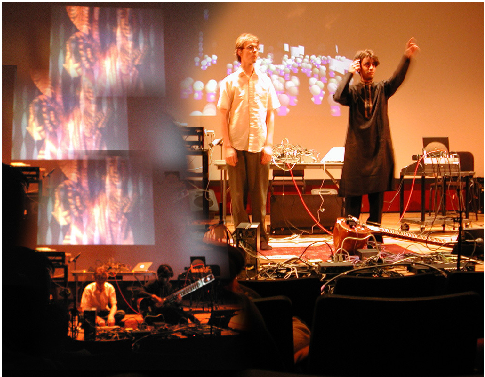
\includegraphics[width=78mm]{img-10-eps-converted-to-crop.pdf}      
\caption{The ESitar in live performance.}
\label{Kapur:img-10}       % Give a unique label
\end{figure}


\section{CONCLUSION}

We have presented a real-time device for sitar performance. The sitar controller captures gestural data from a performer, and uses it to manipulate sounds and visuals. A performer can now use a laptop with a sitar in order to create a multimedia experience for a live audience, using traditional Indian classical sitar technique. Performance based visual feedback provides another means of expression for the performer, as well as a pedagogical tool. In the future we plan to use the ESitar as a tool to transcribe Indian Classical music.


\begin{acknowledgement}
We would like thank Bill Verplank, Michael Gurevich, Scott Wilson, and Max Mathews for their workshop at CCRMA on controllers and the Atmel microprocessor. We would also like that Asha Kapur, Dolly and Surinder Vohra for bringing a sitar from India to build the ESitar with. We would also like to thank Ustad Siraj Khan of the Mewati gharana for his training in the traditional classical theory and technique of sitar performance. Other thanks to Andrew Schloss, Peter Driessen, George Tzanetakis, Tae Hong Park, Dan Trueman, Curtis Bahn, Pavan Vohra, Sona Vohra, Meera Kapur, and Arun Kapur, for their support and inspiration.
\end{acknowledgement}


\section*{Author Commentary: Extended Performance, Modern Pedagogy And Symbiotic Mechatronic Control on the Electronic Sitar}


\paragraph{Ajay Kapur}

The ESitar project started as a simple idea of bringing together all the wonderful advancements of Computer Music technology that  were being applied to Western music and non-western instruments, namely Indian Classical musical instruments. The idea of the ``HyperInstrument'' emerged with the Piano, Cello, Violin, Guitar, and even Saxophone and so much rich data was being collected for augmented and extended performance techniques. Taking these ideas to Raga and Tala with the series of KarmetiK instruments started an entire lifetime of research and artistic pursuit. Three lessons emerged from the building the ESitar, which I now take when creating any new musical instrument:

(1) Practicing your Interface: It has now been over 10 years since I built the first edition of the ESitar. One major success of this invention is that I always have one of my ESitars sitting open, in my studio, ready to play. This is the key to actually practicing the instrument and inventing new ways of performing with it on stage.  I no longer play sitar; I play the ESitar. I cannot imagine getting on stage with a sitar without sensors on it! I would have no idea what to do! The idea of not being able to bend my instrument forward to trigger a sustained reverb. I can't imagine not being able to play a synthesizer with just my frets. I can't imagine not being able to wah-wah my audio from my live sitar, with the thumb pressure of my right hand! I would be naked! There has been four iterations on the design of the ESitar, each learning from the previous version, and each being pushed by new compositional motivations. This is how you build an instrument that stays with you for life. You practice it. 

(2) Mining for Meaning: During my Ph.D., I quickly realized that because I had an instrument with sensors, I could solve research problems being asked in the Music Information Retrieval field, with much more accuracy and in real-time with my multimodal sensor solution. This allowed me to turn my ESitar into a system that knew what tempo I was playing \cite{Benning:2007}
, what pitch I was playing \cite{Kapur:2007}, what section in a composition I was in \cite{Eigenfeldt:2008}, and what emotional state I was in,  all in real-time. This data is essential for the preservation techniques our team was building for Indian Classical music. Most music masters are only preserved by audio recordings. But this is not enough! What fret did they make that note? What posture were they sitting in? What angle was the instrument? All this information is essential to preservation and to building future pedagogical systems in the future. This has spawned an entire field of research from my Ph.D. students studying multimodal techniques for musical data analysis and pedagogy. There is so much more you can do with a NIME than just perform on stage. 

(3) Human to Mechatronic Performance:  One of the most important features of building the ESitar was the ability to communicate with my first robot, the MahaDeviBot. I could never have accomplished the deep interaction techniques with the mechatronic instrument by just using audio analysis. In a way, though lots of machine learning techniques have been experimented with in the lab and on stage, I feel that through my ESitar I am able to extend my control to an entire array of mechatronic musical actuators placed all around a concert hall. After exploring this as a solo musician for years, my true aesthetic goals were accomplished when creating the KarmetiK Machine Orchestra \cite{Kapur:2011}, and building a framework to teach other artists and composer/performers to collaborate in this space together. This symbiotic relationship between humans with NIME's and an Orchestra of 20 different musical mechatronic instruments with over 300 moving actuators was the beginning of a movement that will take our team decades to continue to explore. 

In summary, NIME has evolved from just building instruments, to using new instruments to gather data to do advance music research that pushes pedagogical tools into the future as well  creating new expressive music with the maturity of these instruments now lasting years and even decades as the field has evolved.


\section*{Expert Commentary: Old Lessons for New ``Instruments''}


\paragraph{Dan Trueman}


As we know, the designer of digital musical instruments is invited to completely rethink the relationship between body and sound. No longer constrained by the physics of vibrating strings and resonators, the designer can freely imagine how the body might initiate and modulate sound; the prospect of ``any sound you can imagine'' always lies just around the proverbial corner, and we can't wait to get our hands on it. 

And therein lies the problem: how exactly should we ``get our hands on it?'' And, really, how do we ``imagine'' sound, apart from what we already know in the world, and apart from our bodies? These are tough questions that don't yield easily, and they require inquiry from as many vantage points as possible, whether that be building entirely new instruments ``from scratch'' (like Serge de Laubier's ``meta-instrument'' \cite{Laubier:1998}), accessing the body or nervous system directly (the Hands \cite{Waisvisz:1985}, or the Biomuse system \cite{Knapp:2009}), or reinventing very old instruments (Jeff Snyder's virtually just-intoned Contravielle and Birl, for instance \cite{Snyder:2010}). 

Kapur's electronic sitar represents a particularly strong case of yet another widely-used approach, the so-called ``hybrid'' digital instrument. Sometimes this manifests itself in fairly crude, if effective, ways: put a couple sensors on just about any existing instrument, create a basic mapping from sensor to sound or signal processing, and voil\`{a}, we have a new hybrid instrument that might just be well worth some time and effort. Pre-existing instruments that have drawn the sustained attention of musicians over decades and centuries (or millennia, in the case of the sitar!) have so much to offer, they are natural starting points for exploring digital instrument design and provide clues as to what sorts of connections between body and sound are particularly compelling; the design of the violin, for instance, is much more than an awkward compromise between human body and resonating body. Simply putting a couple sensors on one of these instruments might get us pretty far, if only because these instruments are already so rich to begin with, but Kapur et al. went much further, carefully designing a multifaceted system that was informed by the rich history and performance practices of the sitar, while not remaining confined by these practices. 

Consider, for instance, their approach to capturing what the sitarist's hands are doing. For the left hand, an array of circuits identify which fret is being played while a contact microphone and pitch detection quantifies the all-important pulling and detuning of the string; this combination captures much more than either element could on its own. And for the right hand, a pair of condenser microphones embedded in the bridge of the instrument combine with a force-sensing-resistor (FSR) under the thumb to capture pluck time and direction; I am particularly intrigued by the careful placement of the FSR, which serves to identify pluck direction, but would seem, since this thumb is a crucial fixed connection between body and instrument, to offer the potential to reveal much more. This is a rich and multifaceted sensor array, and it is not hard to imagine how it might be used with a contemporary machine-learning mapping system like Rebecca Fiebrink's Wekinator \cite{Fiebrink:2009}. At the time, Kapur mapped it to a variety of things, some immediately ``instrumental'' in character, others more ``accompanimental'' in nature (like drones and tabla riffs), and others yet further afield, like visuals.


I had the great privilege of performing alongside Kapur and his ESitar shortly after it was built. One of the compelling things about his hybrid instrument is that it is hybrid in multiple ways; yes it is a hybrid digital and acoustic instrument, but it is also a hybrid instrument and system. Playing with him felt like playing with an instrumentalist, but also, say, an airline pilot; he was driving a system that had its own momentum, its own sources of energy, while also subtly manipulating an instrument that was immediately responsive to the nuanced expressive variations of his playing. In some ways, it is this latter hybridity that is so new and exciting about digital instruments; our ``instruments'' can take on lives of their own in ways that acoustic ones simply can't, and these systems offer unprecedented compositional and design possibilities. Even this many years after the ESitar was built, it feels like we are at the beginning of something new and exciting, where the lessons from these beautiful old instruments continue to inform and inspire our construction of new instruments and systems.

